%        File: qspn.tex
%     Created: Fri Oct 13 09:00 PM 2006 C
% Last Change: Fri Oct 13 09:00 PM 2006 C
%
\documentclass[a4paper]{article}
\usepackage{color,graphicx}
\usepackage{amsmath}
\usepackage{amsthm}
\usepackage{amssymb}
\usepackage{amsfonts}
\RequirePackage{ifpdf} % running on pdfTeX?
\ifpdf
\usepackage[pdftex]{hyperref}
\else
\newcommand{\href}[2]{ #1 }
\fi
\title{Quantum Shortest Path Netsukuku}
\author{AlpT (@freaknet.org)}
\begin{document}
\maketitle

\begin{abstract}
	This document describes the QSPN, the routing discovery algorithm used
	by Netsukuku.
	Through a deductive analysis the main proprieties of the QSPN are
	shown. Moreover, a second version of the algorithm, is presented.
\end{abstract}

\section{Preface}
\label{sec:preface}

The first part of the document describes the reasoning which led us to the
construction of the current form of the QSPN v2.
If you are just interested in the description of the QSPN v1 and v2 and you
already know the concept of the Tracer Packet, you can directly skip to
section \ref{sec:CTP}.

\section{The general idea}
\label{sec:general_idea}

The aim of Netsukuku is to be a (physical) scalable mesh network, completely
distributed and decentralised, anonymous and autonomous.

The software, which must be executed by every node of the net, has to be
unobtrusive. It has to use very few CPU and memory resources, in this way it
will be possible to run it inside low-performance computers, like Access Points,
embedded devices and old computers.

If this requirements are met, Netsukuku can be easily used to build a worldwide
distributed, anonymous and not controlled network, separated from the
Internet, without the support of any servers, ISPs or control authorities.

\subsection{The network model}
\label{sec:net_model}

Netsukuku prioritises the stability and the scalability of net: the network
has to be able to grow to even $2^{2^7}$ nodes.

A completely dynamic network would requires rapid and frequent updates
of the routes and this is in contrast with the stability and the scalability
requirements of Netsukuku.
For this reason, we restrict Netsukuku to the case where a node won't change
its physical location quickly nor often.

This assumption is licit, because the location of a wifi node mounted on
top of a building won't change and its only dynamic actions would be the
joining and the disconnection to and from the network and the changes of the
quality of its wifi links.
However, there are some consequences of this assumption:
\begin{enumerate}
	\item	Mobiles node aren't supported by Netsukuku algorithms.
		\footnote{It is possible to use other mesh network protocols
		designed for mobility in conjunction with Netsukuku, in the
		same way they are used in conjunction
		with the Internet (f.e. see \href{http://olsrd.org}{olsrd}). }
	\item   The network isn't updated quickly: several minutes may be
		required before all the nodes become aware of a change of the
		network (new nodes have joined, more efficient routes have
		become available, \dots). However, when a node joins
		the network, it can reach all the other nodes from the first
		instant, using the routes of its neighbours.
\end{enumerate}


\subsection{The routing algorithm}
One of the most important part of Netsukuku, is the routing discovery
algorithm, which is responsible to find all the most efficient routes of the
network. These routes will permit to each node to reach any other node.

The routing algorithm must be capable to find the routes without overloading
the network or the nodes' CPU and memory resources.

\subsection{The QSPN}

Netsukuku implements its own algorithm, the \emph{QSPN} (\textbf{Q}uantum
\textbf{S}hortest \textbf{P}ath \textbf{N}etsukuku). The name derives from the
way of working of its principal component: the \emph{TP} (Tracer Packet), a
packet which gains a ``quantum'' of information at each hop.

The QSPN is based on the assumptions described in section \ref{sec:net_model}.

\section{Network topology}
\label{sec:net_topology}

The QSPN alone wouldn't be capable of handling the whole network, because it
would still require too much memory. For example, even if we store just one
route to reach one node and even if this route costs one byte, we would need
1Gb of memory for a network composed by $10^9$ nodes (the current Internet).

For this reason, it's necessary to structure the network in a convenient
topology.

\subsection{Fractal topology}
Netsukuku, adopts a fractal like structure:
256 nodes are grouped inside a \emph{group node} (gnode), 256 group nodes are grouped
in a single \emph{group of group nodes} (ggnode), 256 group of group nodes are
grouped in a gggnode, and so on.
(We won't analyse the topology of Netsukuku. You can find more information
about it in the main documentation: \cite{ntksite}).
\newline
Since each gnode acts as a single real node,
the QSPN is able to operate independently on each level of the fractal.

Because in each level there are a maximum of 256 (g)nodes, the QSPN will
always operate on a maximum of 256 (g)nodes, therefore we would need just to
be sure that it works as expected on every cases of a graph composed by $\le
256$ nodes. By the way, we'll directly analyse the general case.

For the sake of simplicity, in this paper, we will assume to operate on level
0 (the level formed by 256 single nodes).

\section{Tracer Packet}
\label{sec:TP}

A \emph{TP} (Tracer Packet) is the fundamental concept on which the QSPN is
based: 
it is a packet which stores in its body the IDs of the traversed hops.

\subsection{Tracer Packet flood}
\label{sec:TP_flood}

A TP isn't sent to a specific destination but instead, it is used to flood the
network. By saying ``the node A sends a TP'' we mean that ``the node A is
starting a TP flood''.

A TP flood passes only once through each node of the net: a node which
receives a TP will forward it to all its neighbours, except the one from which
it received the TP. Once a node has forwarded a TP, it will not forward any
other TPs of the same flood.

\subsection{Proprieties of the tracer packet}
\begin{enumerate}
	\item A node $D$ which received a TP, can know the exact route covered
		by the TP. Therefore, $D$ can know the route to reach the
		source node $S$, which sent the TP, and the routes to reach
		the nodes standing in the middle of the route.
		
		For example, suppose that the TP received by $D$ is: $\left\{
		S, A, B, C, D \right\}$. By looking at the packet $D$ will
		know that the route to reach $B$ is $C\rightarrow B$, to reach $A$ is
		$C\rightarrow B\rightarrow A$, and finally to reach $S$ is
		$C\rightarrow B\rightarrow A\rightarrow S$.
		The same also applies for all the other nodes which received
		the TP, f.e, $B$ knows that its route to reach $S$ is
		$A\rightarrow S$.
	\item Suppose that $S$ sends a TP. The first TP of this flood received
		by a generic node $D$, will be the TP which covered the
		fastest route which connects $S$ to $D$.
		The fastest $S \rightarrow D$ route is the route with the
		minimum \emph{rtt} (Round-Trip Time) between $S$ and $D$.
\end{enumerate}


\subsubsection*{Example}
\begin{figure}[h]
	\begin{center}
		\includegraphics[scale=0.4]{fig/segABCDEF}
	\end{center}
	\caption{A simple graph}
\end{figure}

Suppose that $D$ sends a TP. The TP will cover this routes:
$D \rightarrow E \rightarrow F$ and $D \rightarrow C \rightarrow B \rightarrow A$.
When the TP reaches the node $F$ and the node $A$, the flood will stop,
because either $A$ and $F$ won't be able to forward the TP to any other node.

At the end, $A$ will know the route $A \rightarrow B \rightarrow C \rightarrow D$ and $F$ will know the
route $F \rightarrow E \rightarrow D$.

\section{Routes of a graph}
\label{sec:gen_routes}

Given a graph $\mathbf{G}$ we want to find all the existing routes between a node and
all the other nodes.

Let $N$ be a generic node. Starting from $N$ we explore the entire graph
until we re-enter in a cycle already visited or we cannot proceed any further.
This approach is similar to the Depth-First Search\cite{DFS} algorithm, but instead of
searching for a specific goal, we just traverse the entire graph.
Note that a cycle is traversed only once, because we need non redundant
routes. In other words, if we already know the $S \rightarrow A \rightarrow B
\rightarrow C \rightarrow D$ route,
it's useless to known that we can reach $D$ with the $S \rightarrow A
\rightarrow B \rightarrow C \rightarrow A \rightarrow B \rightarrow C
\rightarrow D$ route.

This is the pseudo code of the algorithm:

\begin{verbatim}
generate_routes(G) {
        forall node in G
                /* Starts the exploration of the graph from the ``node'' of the
                   graph ``G'' and print all its routes */
                walk(node, node)
}

/* Print all the routes which start from the node `N' */
walk(N, branch) {
        deepened=0

        forall L in N.links
                /* L is a neighbour of N */

                if(L in branch)
                        /* If ``L'' is already contained in the explored
                           branch, we've found a cycle. Since we just need to
                           traverse only once a cycle, we skip this ``L'' node
                           and continue to consider the other neighbours
                           of N */
                        continue;

                newbranch=branch + L    /* Append in the explored branch the
                                           ``L'' node. */

                walk(L, newbranch)      /* Recursively  explore the new
                                           branch */
                
                /* Indicate that we've deepened in the graph at least once */
                deepened=1

        if(!deepened)
                /* We haven't deepened in the above for, this means that the
                   current branch can't be explored anymore, therefore it is a
                   valid route. Print it */
                print branch
}
\end{verbatim}

A proof of concept of the above algorithm has been implemented in Awk
\cite{genrouteawk}.

\subsection*{Example}
Consider this graph:

\begin{figure}[h]
	\begin{center}
		\includegraphics[scale=0.4]{fig/cycleABCD_E}
	\end{center}
	\caption{A simple graph with one segment and one cycle}
	\label{fig:gen_route_sample}
\end{figure}

Given this graph as input the algorithm will output:
\label{sec:genroute_output}
\begin{align*}
& A \rightarrow B \rightarrow D \rightarrow C\\
& A \rightarrow B \rightarrow D \rightarrow E\\
& A \rightarrow C \rightarrow D \rightarrow B\\
& A \rightarrow C \rightarrow D \rightarrow E\\
& B \rightarrow A \rightarrow C \rightarrow D \rightarrow E\\
& B \rightarrow D \rightarrow C \rightarrow A\\
& B \rightarrow D \rightarrow E\\
& C \rightarrow A \rightarrow B \rightarrow D \rightarrow E\\
& C \rightarrow D \rightarrow B \rightarrow A\\
& C \rightarrow D \rightarrow E\\
& D \rightarrow B \rightarrow A \rightarrow C\\
& D \rightarrow C \rightarrow A \rightarrow B\\
& D \rightarrow E
\end{align*}

\section{Raw Tracer Packet flood}
\label{sec:raw_TP_flood}

We can consider each route given by the output of the above algorithm as a
single Tracer Packet.
In fact, it is possible to implement the same algorithm using a slightly
modified version of the TP flood, called the Raw TP flood (the name explains
why it isn't used by the QSPN):

The flood is not restricted like in a normal TP flood: one or more Raw TP can
pass from the same node. The end of the flood is given by this rule: a node
will not forward to any of its neighbours the RTP if its ID is already present
in the route contained in the body of the packet.
Finally, like in the normal TP, a node doesn't forward the RTP to the
neighbour from which it has received the packet itself.

If every node of the network sends a Raw TP flood, then every node will get
all the possible routes to reach any other node.
\newline
As you can see, the RTP flood performs a ``live'' version of the algorithm
described in section \ref{sec:gen_routes}.
Obviously this is far from an efficient routing discovery algorithm, but it
represents a good start.

\section{Routes simplification}
\label{sec:simplify_routes}

Looking carefully at the example output (\ref{sec:genroute_output}) of the
Generate Route algorithm, we can notice that many routes are higly redundant,
in other words, some routes are almost the same.
Consider for example the following four routes:
\begin{align}
	& A \rightarrow B \rightarrow D \rightarrow E \label{eq:e1}\\
	& D \rightarrow E \label{eq:e2} \\
	& A \rightarrow B \rightarrow D \rightarrow C \label{eq:e3}\\
	& D \rightarrow C \rightarrow A \rightarrow B \label{eq:e4}
\end{align}

As we've seen in the previous section \ref{sec:raw_TP_flood}, we can consider
these routes as effective Tracer Packets.
In this example, the TP \eqref{eq:e1} cover the same route of the TP
\eqref{eq:e2}. Therefore we can save one TP by just sending the TP
\eqref{eq:e1}, which will traverse the route \eqref{eq:e2} too.

The TP \eqref{eq:e3} covers part of the TP \eqref{eq:e4}, thus we can simplify
the two of them by just sending a TP which cover this route: $A \rightarrow B
\rightarrow D \rightarrow C \rightarrow A \rightarrow B$.

Continuing in this process we can further simplify the two TP:
\[ ABDCAB + ABDE \Rightarrow  ABDCABDE \]

Thus, from the initial four TPs we've found a unique TP which gives the same
routes of the original ones.

\subsection{Simplification rules}
\label{sec:simplification_rules}

We can derive some rules to simplify routes.

Since we can represent a route as a string where each symbol is a node, we can
also describe the routes simplification as a series of operations on strings.

In the following rules, each letter found in an expression represents a generic string,
which may be also the NULL string, f.e. the ``$XX$'' string can be anything like
$foofoo$ or $1234512345$.
\\
The $c\dots c$ expression represents a cycle, where the $c$ character refers
to just one node, and not to an entire string.
\begin{description}
	\item[XY+YZ $\Rightarrow$ XYZ]
		If two routes share respectively the ending and the starting
		part, they can be merged into a unique route. Example:
		\[ABCDE + CDEKRE \Rightarrow ABCDEKRE \]
	\item[YXZ + X $\Rightarrow$ YXZ]
		Example:
		\[123ABCXYZ + ABC \Rightarrow 123ABCXYZ\]
	\item[Xc\dots c + XcY $\Rightarrow$ Xc\dots cY]
		Example:
		\[123ABCDA + 123A987 \Rightarrow 123ABCDA987\]
	\item[c\dots cZ + YcZ $\Rightarrow$ Yc\dots cZ]
		Example:
		\[ABCDA123 + 987A123 \Rightarrow 987ABCDA123\]
	\item[c\dots c + YcZ $\Rightarrow$ Yc\dots cZ]
		Example:
		\[ABCDA + 987A123 \Rightarrow 987ABCDA123\]
	\item[Invalid route]
		A route must not be in the form of:
		\[ XacaY \]
		where $a$ and $c$ are two nodes.
		A simplification, which gives a route of this form, is
		not considered valid. This is because a TP must not change its
		verse while traversing a network.
\end{description}

All these rules can be applied recursively to the routes of a graph, until
they cannot be simplified anymore.

A proof of concept of the above algorithm has been implemented in Awk \cite{simrouteawk}.

\subsection*{Example}
Simplifying all the routes of the example \ref{sec:genroute_output}, we obtain
just these two TPs:
\begin{align}
 &A \rightarrow B \rightarrow D \rightarrow C \rightarrow A \rightarrow B
 \rightarrow D \rightarrow E\\
 &A \rightarrow C \rightarrow D \rightarrow B \rightarrow A \rightarrow C \rightarrow D \rightarrow E
\end{align}

You can verify that all the routes listed in \ref{sec:genroute_output} are
contained in these two simplified TPs.

\subsection{General results}
By looking at many different simplifications, we can recognize some general
rules:
\begin{enumerate}
	\item For each TP there has to be its inverse. For example, if there's
		a TP which covered the route $12345$, then there has to be at
		least the TP which covers the inverse route $54321$.
	\item In a segment, to give all the routes to all the nodes, it is
		sufficient that the two extremes sends a TP. Example:
		\begin{figure}[h]
			\begin{center}
				\includegraphics[scale=0.4]{fig/segABCDEF}
			\end{center}
			\caption{A segment}
		\end{figure}
		in this case, if $A$ and $F$ send a TP, all the routes will be
		generated, since the two TP would be: $ABCDEF$ and $FEDCBA$.
		You can verify that in these two TP, there are contained all
		the routes of the segment.
	\item In a cycle, just two TP are needed, and one is the reverse of
		the other. The first can be constructed in this way: 
		\begin{itemize}
			\item Choose a node of the cycle, this will be the
				pivot node.
			\item Start from one neighbour of the pivot and write
				sequencially all the other nodes until you
				return to the pivot (but do not include it).
				Call this string $C$.
			\item The TP will be:
				\[CpC\]
				where $p$ is the pivot node.
		\end{itemize}
		Example:
		\begin{figure}[h]
			\begin{center}
				\includegraphics[scale=0.4]{fig/cycleABCDEF}
			\end{center}
			\caption{A cycle}
		\end{figure}
		if we choose the node $D$ as the pivot, we can write the TP
		as:
		\[ EFABCDEFABC \]
		and its reverse:
		\[ CBAFEDCBAFE \]
		These two TPs will give all the routes to all the nodes of the
		cycle.
\end{enumerate}

\subsection{The question}

Can we implement a ``live'' version of the Simplify Route algorithm like we
did with the Generate Route one?\\
The reply is ahead ;).

\newpage
\section{Continuous Tracer Packet}
\label{sec:CTP}

A Continuous Tracer Packet (CTP) is an extension of the TP flood: a node will
always forward a TP to all its neighbours, excepting the one from which it has
received the TP.
If a node is an extreme of a segment, i.e. a node with just one link, it will
erase the route stored in the body of the TP and will forward back the TP.

In short, a CTP is a TP flood which will never end, thus it will continue to
explore all the infinite combination of routes. 

\subsection*{Example}
Consider this graph.
\begin{figure}[h]
	\begin{center}
		\includegraphics[scale=0.4]{fig/cycleABC}
	\end{center}
	\caption{The simplest cyclic graph}
	\label{fig:cycleABC}
\end{figure}
If $A$ sends a CTP flood, there will be two CTPs that will explore
respectively these routes:
\[
	 A \rightarrow B \rightarrow C \rightarrow A \rightarrow B \rightarrow
	 C \rightarrow A \rightarrow B \rightarrow C \rightarrow A \rightarrow
	 B \rightarrow C \rightarrow \dots
\]
\[
	 A \rightarrow C \rightarrow B \rightarrow A \rightarrow C \rightarrow
	 B \rightarrow A \rightarrow C \rightarrow B \rightarrow A \rightarrow
	 C \rightarrow B \rightarrow \dots
\]

\subsection{Reflected CTP}
Suppose that the node $N$ has just one link.
$N$, before back forwarding the received CTP, erases the route contained in
the body, because the nodes which precede it already know this same route.
\\
For example, consider this segment:
\[ \cdots -- A -- B -- C -- N \]
If $N$ sent the 
receives the following TP

\section{QSPN v2}
\label{sec:QSPNv2}
The second version of the QSPN\footnote{The short name of the QSPN v2 is
\emph{Qv2}} can be described in a single phrase:

\emph{A Continuous Tracer Packet will continue to roam inside}

\emph{the network until it carries interesting information.}

\subsection{Interesting information}
A node considers a received CTP interesting when its body contains at least a
new route, i.e. a route that the node didn't previously know.
In other words, if a CTP contains routes already known by the node, it is
considered uninteresting.

When a node receives an interesting CTP, it forwards the packet to all its
neighbours, excepting the one from which it has received the CTP.
If, instead, the CTP is uninteresting, it will drop the packet.

Note that if a CTP is uninteresting for the node $N$, then it is also
uninteresting for all the other nodes. This is because an uninteresting CTP
contains routes which has been previously received, memorized and forwarded
by the node $N$, therefore all the other nodes already know the same
routes too.

\subsubsection*{Example}
\label{sec:cycle_qv2_example}

Consider this graph.
\begin{figure}[h]
	\begin{center}
		\includegraphics[scale=0.4]{fig/cycleABC}
	\end{center}
	\caption{The A-B-C-A cycle}
	\label{fig:A-B-C-A}
\end{figure}
Suppose that $A$ sends a CTP. 
The two CTPs, after having covered the following two paths will stop:
\[
A \rightarrow B \rightarrow C \rightarrow A \rightarrow B \rightarrow C
\]
\[
A \rightarrow C \rightarrow B\rightarrow A \rightarrow C \rightarrow B
\]
Let's analyze the first CTP step by step, considering that before $A$ sent the
CTP, none knew any route.
\begin{description}
	\item[A $\rightarrow$ B] At this point $B$ doesn't know any route to
		reach $A$, therefore it considers this CTP as interesting and
		forwards it to $C$.
	\item[A $\rightarrow$ B $\rightarrow$ C] By looking at this packet $C$
		learns a route to reach $B$ and $A$.
	\item[A $\rightarrow$ B $\rightarrow$ C $\rightarrow$ A] The node $A$
		learns a route to reach $C$.
	\item[A $\rightarrow$ B $\rightarrow$ C $\rightarrow$ A $\rightarrow$
		B] The node $B$ learns a route to reach $C$.
	\item[A $\rightarrow$ B $\rightarrow$ C $\rightarrow$ A $\rightarrow$
		B $\rightarrow$ C] Finally, $C$ drops the packet, because it
		already knows all the routes contained in it.
\end{description}

From this example we can derive a general result: a CTP will always terminate
in a cycle.

\subsection{Live routes simplification}
The QSPN v2 is the ``live'' version of the Simplify Route algorithm (section
\ref{sec:simplify_routes}).

The CTP flood of the QSPN v2 explores the entire graph, but unlike the RTP
(section \ref{sec:raw_TP_flood}), it drops the TPs which contains
redundant routes, thus only the simplified, non redundant routes survives and
continue to explore the graph.

\newpage
\subsection{Cyclicity}
\label{sec:CTP_ciclicity}
When a CTP reaches the extremity of a segment, it is forwarded back, thus it's
like the extreme nodes had a link with themself.

\begin{figure}[h]
	\begin{center}
		\includegraphics[scale=0.4]{fig/cycleselfABC}
	\end{center}
	\caption{A segment as viewed from a CTP}
	\label{fig:CTP_segment}
\end{figure}

From the point of view of a CTP, even a segment is a cycle, therefore, for a
CTP, any connected graph is formed just by cycles.

For this reason, a CTP will explore any combination of cycles of the graph.

\subsubsection{Subcycles examples}
These examples highlights some subcycles of a simple graph.

\begin{figure}[h]
	\begin{center}
		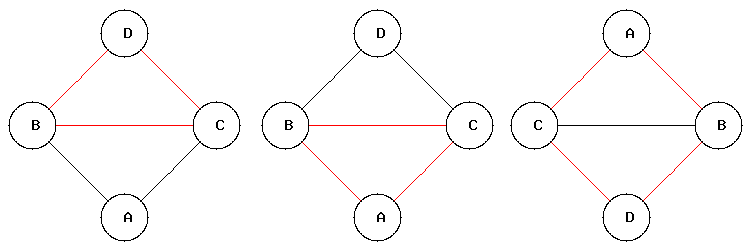
\includegraphics[scale=0.4]{fig/cycleABCD_BC_123}
	\end{center}
\end{figure}


%%%%%%%% TODO: ABCBABCBABCBA

\subsection{Finiteness}
The Qv2 will finish the exploration of the graph in an finite amount of time,
i.e. the flood will terminate.

As you've seen in the example \ref{sec:cycle_qv2_example}, a CTP will always
terminate in a cycle. 
Since every connected graph is a composition of cycles
%% TODO: CONTINUE HERE

\subsection{Routes limit}
%%%%%%%%%%%%%%%%%%%% TODO %%%%%%%%%%%%%%%%%%%%%%%%%%%%


\subsection{Scalability}
%%%%%%%%%%%%%%%%%%%% TODO %%%%%%%%%%%%%%%%%%%%%%%%%%%%
TODO: Il primo TP ricevuto ha percorso la rotta migliore
Il formato della mappa interna cambia!


\section{QSPN v1}
\label{sec:QSPNv1}
%%%%%%%%%%%%%%%%%%%% TODO %%%%%%%%%%%%%%%%%%%%%%%%%%%%
La prima fase (qclose) equivale a un CTP normale.
Appena 
Un TP normale non genera mai rotte ridondanti.

Il v1 usa meno memoria del v2.

\subsection{Rtt and bandwidth}
%%%%%%%%%%%%%%%%%%%% TODO %%%%%%%%%%%%%%%%%%%%%%%%%%%%

Questo discorso vale sia per il v1 che per il v2.
Vedi (Ntk\_rfc\_bandwidth) sulla tecnica del misuramento dei link.
Bisogna necessariamente ritardare il forwarding, altrimenti potrebbero essere
non considerate alcune rotte.
Il ritardo prende le rotte medie di bw e rtt. Il difetto e' che vengono
scartate le rotte estreme.

\section{Asymmetric bandwidth}
Bla. Bla.
Vedi --> Ntk\_rfc\_bandwidth.
%%%% Mandare in lista la risposta al tizio che aveva chiesto sulla questione
%%%% }dell'asimmetria


%%%%%%%%%%%%%%%%
% Bibliography %
%%%%%%%%%%%%%%%%

\begin{thebibliography}{99}
	\bibitem{ntksite} Netsukuku website:
		\href{http://netsukuku.freaknet.org/}{http://netsukuku.freaknet.org/}.
	\bibitem{DFS} Depth-First Search:
		\href{http://en.wikipedia.org/wiki/Depth-first\_search}{http://en.wikipedia.org/wiki/Depth-first\_search}.
	\bibitem{genrouteawk} Generate Routes in Awk:\\
		\href{http://cvs.hinezumi.org/viewcvs/netsukuku/proto/qspn/generate\_routes.awk}{generate\_routes.awk}.
	\bibitem{simrouteawk} Simplify Routes in Awk:\\
		\href{http://cvs.hinezumi.org/viewcvs/netsukuku/proto/qspn/simplify\_routes.awk}{simplify\_routes.awk}.
\end{thebibliography}

\end{document}
